\newpage
\subsection{ACAS-X like Reach Set Approximation}\label{s:acasReachSet}

\paragraph{Summary:} This procedure will produce trajectories encoding ACAS-X separation modes, ideal for controlled airspace navigation. 

\paragraph{Motivation:} The implementation of \emph{ACAS-Xu} behavior in DAA system will  be mandatory for \emph{National Airspace System Integration} in United spaces \cite{shively2018uas}. 

Implementation of ACAS-Xu like behavior increase usability of approach, if it can be achieved without major concept changes.


\paragraph{Background:} The \emph{ACAS-Xu} system on the operational level has been described in \cite{marston2015acas}. The \emph{Policy for Collision Avoidance} proposal has been given in \cite{julian2016policy}.

Some behavioral patterns can be encoded into  \emph{Reach Set}. ACAS-Xu navigation part is basically \emph{Look-up table of Maneuvers for Allowed Separations}.
 
The \emph{Evasive Maneuver} selection process in ACAS-Xu is similar to our approach: \emph{Select most energy efficient maneuver in compliance with space-time constraints}. ACAS-Xu intruder model is similar to our \emph{Body Volume Intersection Model} (app. \ref{s:bodyvolumeIntersection}). The \emph{ACAS-Xu} defines following base separations:

\begin{enumerate}
    \item \emph{Horizontal} - movements on a \emph{Horizontal Plane} in \emph{Global Coordinate System}.
    
    \item \emph{Vertical} - movements on a \emph{Vertical Plane} in \emph{Global Coordinate System}.
    
\end{enumerate}

\noindent There are allowed custom separations which can be used, for further experimentation: 
\begin{enumerate}
    \item \emph{Slash} - movement on $+45^{\circ}$ \emph{Tilted Plane to Horizontal Plane} in \emph{Global Coordinate System}.
    
    \item \emph{Backslash} - movement on $-45^{\circ}$ \emph{Tilted Plane to Horizontal Plane} in \emph{Global Coordinate System}.
    
\end{enumerate}

\noindent For given \emph{Movement Automaton} implementation (sec. \ref{s:modelMAImplementation}) the separations are given as follow:

\begin{equation}\label{eq:implementedseparations}
    \begin{aligned}
        Horizontal & = \{Straight, Left, Right \}\\
        Vertical & = \{Straight, Up, Down\}\\
        Slash & = \{Straight, UpLeft, DownRight\}\\
        Backslash & = \{Straight, UpRight, DownLeft\}\\
    \end{aligned}
\end{equation}

\noindent For each $Node(\dots,buffer)$ and each \emph{separation} there is a evaluation function $isSeparation$ which decides, if \emph{Trajectory} defined by node buffer is made up only from \emph{Separation} movements.  The function $isSeparation(\dots)$ is defined like:

\begin{equation}\label{eq:isSeparationPredicate}
    isSeparation(buffer,separation) =
    \begin{cases}
        \begin{aligned}
            \forall & movement \in buffer,\\ & movement \in separation
        \end{aligned}&: true\\
        otherwise &: false
    \end{cases}
\end{equation}

\noindent Following \emph{Separation Modes} can be defined with given \emph{separations}:

\begin{enumerate}
    \item \emph{Horizontal} (ACAS-X defined mode) containing \emph{horizontal} separation. 
    
    \item \emph{Vertical} (ACAS-X defined mode) containing \emph{vertical} separation.
    
    \item \emph{Horizontal-Vertical} (ACAS-X defined mode) containing \emph{horizontal, vertical} separations.
    
    \item \emph{Full} (custom defined mode) containing all \emph{Separation Modes}.
    
\end{enumerate}

\begin{note}
    Every separation modes generate 2D trajectories set on \emph{Respective plane}. There is no need for \emph{Tuning parameters} for further \emph{Expansion Constraint}.    
\end{note}

\paragraph{Expansion Constraint Function Implementation} (alg. \ref{alg:ExpansionConstraintFunctionForACASLikeReachSet}) is based on the simple principle:
\emph{Select only candidate Nodes which Trajectories have at least one desired Separation Mode}.

\paragraph{Step: Initialization} sets candidate \emph{Nodes} as the empty set,  leftover \emph{Nodes} as the empty set, and, select all nodes to form a \emph{stack} which represents \emph{Finishing Trajectories} in working $cell_{i,j,k}$,

\paragraph{Step: Candidate Selection Process} is evaluated for each \emph{test Node} from \emph{passing Node Set}. 

For each \emph{applicable separation}, given as input parameter \emph{separations}, The test function \emph{isSeparation} (eq. \ref{eq:isSeparationPredicate}) is applied:
\begin{enumerate}
    \item If \emph{test Node} trajectory belongs to at least one allowed separation it is added to candidates set.
    \item Else is added to \emph{Leftovers}.
\end{enumerate}

\begin{note}
    \emph{Separation sets} (eq. \ref{eq:implementedseparations}) are not \emph{exclusive sets} in \emph{Movement Automaton} domain. One \emph{Trajectory} contained by Node can belong to multiple \emph{Separations}.    
\end{note}

\begin{algorithm}[H]
\SetKwInOut{Input}{Input}\SetKwInOut{Output}{Output}\SetKwInOut{TuningParameters}{Tuning Parameters}
    \Input{Node[] stack, Cell cell$_{i,j,k}$, Separation[] separations}
    \TuningParameters{$None:\varnothing$}
    \Output{Node[] candidates, Node[] leftovers}
    
    \BlankLine
    \# Initialize structures\;
    Node[] candidates = [], Node[] leftovers=[]\;
    Node[] passing = cell$_{i,j,k}$.getFinishingTrajectories(stack)\;
    
    \BlankLine
    \# Select nodes containing trajectories with usable separations\;
    \For{Node test $\in$ passing}{
        \For{separation $\in$ separations}{
            \BlankLine
            \# Get separations for Node\;
            Separations[] nodeSeparations = test.getSeparations()\;
            \BlankLine
            \# If trajectory given by buffer is on Separation plane\;
            \If{isIn(isSeparation(test.buffer,separation)(\ref{eq:isSeparationPredicate})}{
                candidates.append(test)\;
            }
        }
        \BlankLine
        \# If there was no applicable separation, throw Node away\;
        \If{test $\not\in$ candidates}{
            leftovers.append(test)\;
        }
    }
    \BlankLine
    \# Return results\;
    \Return{[candidates,leftovers]}
    
    \caption{Expansion Constraint function for \emph{ACAS-like Reach Set Approximation}}
    \label{alg:ExpansionConstraintFunctionForACASLikeReachSet}    
\end{algorithm}

\paragraph{Example:} for \emph{Avoidance Grid} with \emph{Distance 10 m}, \emph{Layer count 10}, \emph{Horizontal range $[-45^\circ,+45^\circ]$}, \emph{Horizontal Cell Count 7}, \emph{Vertical range $[-30^\circ,+30^\circ]$}, and \emph{Vertical Cell Count 5}. Is given in (fig. \ref{fig:acasLikeReachSetVariousSeparationMode}). The UAS is at \emph{Back-side} of \emph{Figure} (initial state is at all \emph{Trajectory Origins}). The \emph{black dashed line} marks \emph{Avoidance Grid} space boundary. Each trajectory has its own color and ends at \emph{Front-side} of \emph{Avoidance Grid Boundary}.

\emph{Full} separation mode is given in (fig. \ref{fig:acasLikeReachSetFull}). \emph{Horizontal-Vertical} separation mode, used in original \emph{ACAS-Xu} testing \cite{marston2015acas}, given in (fig. \ref{fig:acasLikeReachSetHorizontalVertical}). \emph{Horizontal} separation mode given in (fig. \ref{fig:acasLikeReachSetHorizontalOnly}) is usually used by planes. \emph{Vertical} separation mode given in (fig. \ref{fig:acasLikeReachSetVerticalOnly}) is usually used by copters.

\begin{figure}[H]
	\centering
    \begin{subfigure}{0.48\textwidth}
        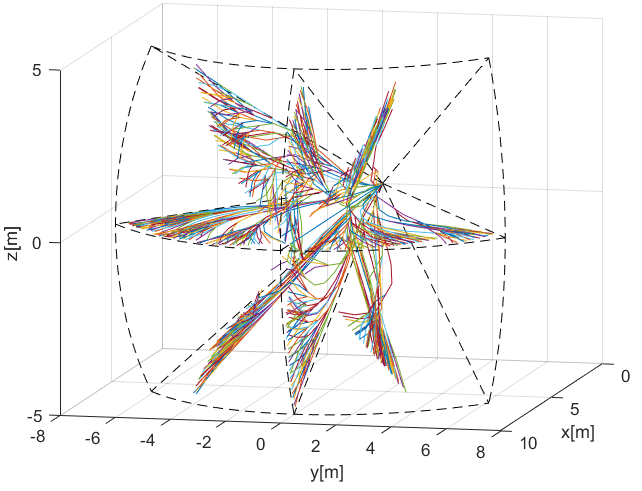
\includegraphics[width=0.9\linewidth]{\FIGDIR/RS005ACASLikeReachSetEstimationMethodFull}
        \caption{Full.}
        \label{fig:acasLikeReachSetFull}
    \end{subfigure}
    \begin{subfigure}{0.48\textwidth}
        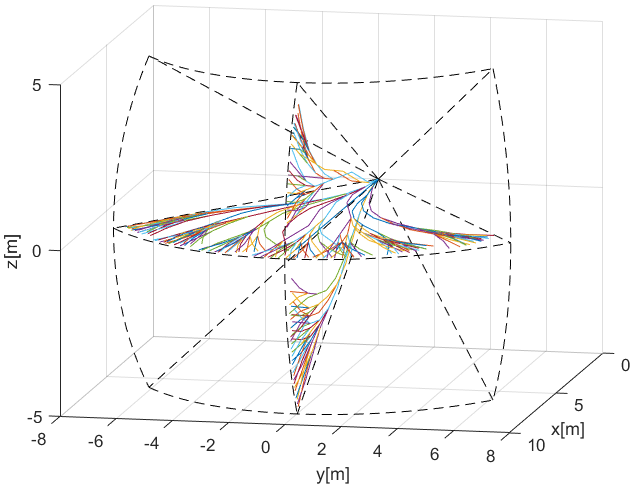
\includegraphics[width=0.9\linewidth]{\FIGDIR/RS006ACASLikeReachSetEstimationMethodHorizontalVertical} 
        \caption{Horizontal-Vertical.}
        \label{fig:acasLikeReachSetHorizontalVertical}
    \end{subfigure}
    \\
    \begin{subfigure}{0.48\textwidth}
        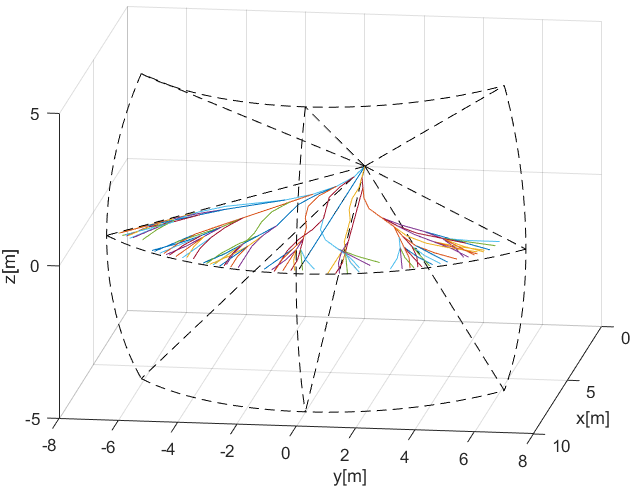
\includegraphics[width=0.9\linewidth]{\FIGDIR/RS008ACASLikeReachSetEstimationMethodHorizontal} 
        \caption{Horizontal.}
        \label{fig:acasLikeReachSetHorizontalOnly}
    \end{subfigure}
    \begin{subfigure}{0.48\textwidth}
        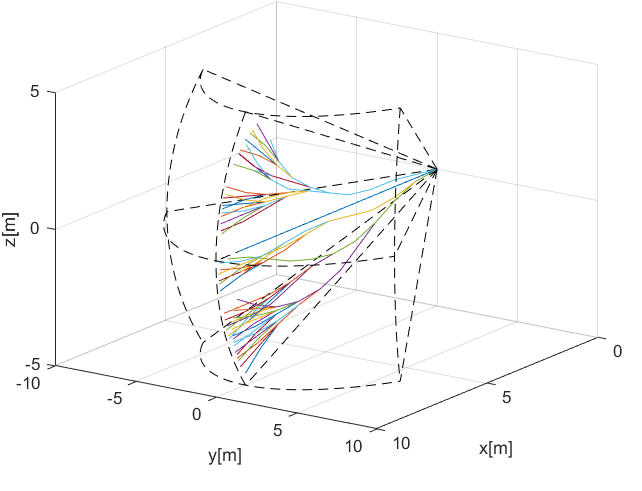
\includegraphics[width=0.9\linewidth]{\FIGDIR/RS009CASLikeReachSetEstimationMethodVertical} 
        \caption{Vertical.}
        \label{fig:acasLikeReachSetVerticalOnly}
    \end{subfigure}
    \caption{ACAS-X imitation \emph{reach set} approximation for various \emph{separation modes}. }
    \label{fig:acasLikeReachSetVariousSeparationMode}
\end{figure}

\paragraph{Pros and Cons:} It can be seen from examples (fig. \ref{fig:acasLikeReachSetVariousSeparationMode}) that \emph{ACAS-like Reach Set Approximation Method} (alg. \ref{alg:ExpansionConstraintFunctionForACASLikeReachSet}) generates a full reach set for 2D plane located in 3D space. 

The \emph{Reach Set} contains trajectories with \emph{high coverage ratio} and \emph{high smoothness rating} for selected 2D separation plane. Overall performance compared to full 3D reach sets (sec. \ref{s:chaoticReachSet}, \ref{s:harmonicReachSet} \ref{s:combinedReachSet}) is poor. 

The \emph{node} and \emph{trajectory} count boundary was not implemented. It is common knowledge that \emph{2D} avoidance sets do not require scaling \cite{marston2015acas}. Otherwise, trajectory footprint mechanism like in \emph{Turn-Minimizing Reach Set Approximation} (alg. \ref{alg:ExpansionConstraintFunctionForHarmonicReachSet}) can be introduced.

This reach set implements \emph{Planar-Separation} as a native feature, it can be used for both \emph{navigation} and \emph{avoidance} tasks in \emph{Controlled Airspace}. For \emph{Non-controlled Airspace}, there are far more superior \emph{Combined Reach Set} (sec. \ref{s:combinedReachSet}).
